%%%%%%%%%%%%%%%%%%%%%%%%%%%%%%%%%%%%%%%%%%%%%%%%%%%%%%%%%%%%%%%%%%%%%%%%%%%%%%%%
\documentclass[12pt,conference]{ieeeconf} %Github
\documentclass[12pt,conference]{ieeeconf} %Github
%\documentclass[letterpaper, 12 pt, onecolumn]{ieeeconf} %Prof. Parallel

% Comment this line out
                                                          % if you need a4paper
%\documentclass[a4paper, 10pt, conference]{ieeeconf}      % Use this line for a4
                                                          % paper

\IEEEoverridecommandlockouts                              % This command is only
                                                          % needed if you want to
                                                          % use the \thanks command
\overrideIEEEmargins
% See the \addtolength command later in the file to balance the column lengths
% on the last page of the document

% The following packages can be found on http:\\www.ctan.org
\usepackage{graphics} % for pdf, bitmapped graphics files
\usepackage{epsfig} % for postscript graphics files
%\usepackage{mathptmx} % assumes new font selection scheme installed
%\usepackage{times} % assumes new font selection scheme installed
\usepackage{amsmath} % assumes amsmath package installed
\usepackage{amssymb}  % assumes amsmath package installed

\usepackage{tikz}
\usetikzlibrary{shapes, arrows.meta, positioning}

\usepackage{url}
\usepackage[ruled, vlined, linesnumbered]{algorithm2e}
%\usepackage{algorithm}
\usepackage{verbatim} 
%\usepackage[noend]{algpseudocode}
\usepackage{soul, color}
\usepackage{lmodern}
\usepackage[hidelinks]{hyperref}
\usepackage{fancyhdr}
\usepackage[utf8]{inputenc}
\usepackage{fourier} 
\usepackage{array}
\usepackage{pgf}
\usepackage{makecell}
\usepackage[sorting=none]{biblatex} % For biblatex
\addbibresource{reference.bib} % Path to your .bib file

\SetNlSty{large}{}{:}

\renewcommand\theadalign{bc}
\renewcommand\theadfont{\bfseries}
\renewcommand\theadgape{\Gape[4pt]}
\renewcommand\cellgape{\Gape[4pt]}

\newcommand{\rework}[1]{\todo[color=yellow,inline]{#1}}

\makeatletter
\newcommand{\rom}[1]{\romannumeral #1}
\newcommand{\Rom}[1]{\expandafter\@slowromancap\romannumeral #1@}
\makeatother

\pagestyle{plain} 

\title{GATTO: Can Topological Information Improve Node Classification via GAT?\\
\large Proposal for Learning from Network's project \\}

\author{Francesco Biscaccia Carrara, Riccardo Modolo, Alessandro Viespoli % <-this % stops a space 
\\\\ Master Degree in Computer Engineering \\
University of Padova \\
}

\begin{document}

\maketitle
\thispagestyle{plain}
\pagestyle{plain}

%%%%%%%%%%%%%%%%%%%%%%%%%%%%%%%%%%%%%%%%%%%%%%%%%%%%%%%%%%%%%%%%%%%%%%%%%%%%%%%%
\section{MOTIVATION} 
Node classification is an important topic in graph analysis for assigning to each node a label from a set of predefined classes. \\
Our intention is to see whether pre-computing features obtained via graph embedding and clustering can improve node classification via graph attention networks (GAT)$^\text{\cite{GAT}}$. 

\section{DATA}
The datasets we will be using are taken from Stanford Network Analysis Project (SNAP)$^\text{\cite{SNAP}}$: 
\begin{table}[h!]
\centering
\renewcommand{\arraystretch}{1.5}
\begin{tabular}{|l|c|c|c|}
\hline
\textbf{Network}           & \textbf{Nodes} & \textbf{Edges} & \textbf{Communities} \\
\hline
email-EU-core  & 1005           & 25571          & 42         \\
com-Amazon     & 334863         & 925872         & 75149    \\
wiki-topcats        & 1791489        & 28511807       & 17364    \\
\hline
\end{tabular}
\end{table}
%%%%%%%%%%%%%%%%%%%%%%%%%%%%%%%%%%%%%%%%%%%%%%%%%%%%%%%%%%%%%%%%%%%%%%%%%%%%%%%%
\section{METHODS}

\subsection{Merge Sort Algorithm}
Merge Sort\cite{von1956new} is a divide-and-conquer sorting algorithm that efficiently sorts data by recursively dividing a dataset into smaller subarrays, sorting them, and then merging the sorted subarrays back together. Developed by John von Neumann in 1945, Merge Sort is well-regarded for its stable sorting behavior and predictable time complexity of $O(n \log n)$, where $n$ is the dataset size.

\begin{algorithm}[h]
\vspace{0.5em}
\caption{Merge Sort}
\KwIn{Array $A$ with indices $start$ to $end$}
\KwOut{Sorted array $A$}
\vspace{0.25em}
\SetAlgoLined
\SetKwFunction{FMain}{MergeSort}
\SetKwProg{Fn}{Function}{:}{}

\SetKwFunction{FMerge}{Merge}
\Fn{\FMerge{$A$, $start$, $mid$, $end$}}{
    $n_1 \gets mid - start + 1$\;
    $n_2 \gets end - mid$\;
    
    $A_L[0 \dots n_1 -1]$, $A_R[0 \dots n_2 -1]$\
    
    \For{$i \gets 0$ \KwTo $n_1-1$}{
        $A_L[i] \gets A_L[start + i]$\;
    }
    \For{$j \gets 0$ \KwTo $n_2-1$}{
        $A_R[j] \gets A_R[mid + j+1]$\;
    }
    $i \gets 0$, $j \gets 0$\;
    $k \gets start$ \;
    \While{$i < n_1$ \textbf{AND} $j <n_2 $ }{
   
        \If{$A_L[i] \leq  A_R[j]$}{
            $A[k] \gets A_L[i]$\;
            $i \gets i+1$\;
        }
        \Else{
            $A[k] \gets A_R[i]$\;
           $j \gets j+1$\;
        }
         $k\gets k+1$\;
    }
}
\vspace{0.5em}
\Fn{\FMain{$A$, $start$, $end$}}{
    \If{$start < end$}{
        $mid \gets \lfloor \frac{start + end}{2} \rfloor$\;
        \FMain{$A$, $start$, $mid$}\;
        \FMain{$A$, $mid + 1$, $end$}\;
        \FMerge{$A$, $start$, $mid$, $end$}\;
    }
}
\end{algorithm}
As show in the pseudocode, the algorithm operates by splitting the input array into two halves, repeatedly doing so until each subarray contains a single element. It then merges these subarrays in a way that results in a sorted array. The merging process is the key to Merge Sort's efficiency, as it combines elements in linear time, leading to its overall $O(n\log n)$ complexity.\par
One of the strengths of Merge Sort is its performance consistency, as it maintains the same complexity in the worst, best, and average cases. However, Merge Sort requires additional space proportional to the size of the input data, which can be a drawback in environments with limited memory.

\subsection{Parallelization of Merge Sort Algorithm}
Due to its nature, there are multiple ways to parallelize the Merge Sort algorithm. One straightforward approach is to leverage the hypercube architecture, which provides efficient parallel processing capabilities. This chapter explores a naive solution based on the Bitonic Sorting Paradigm, implemented on a hypercube network.

\subsubsection{Hypercube Architecture}
A hypercube\cite{boman1990hypercube} is a $d$-dimensional structure with $2^d$ nodes, where each node is connected to $d$ other nodes. The diameter of the hypercube is $\log_2{P}$, where $P$ is the number of processors.\par

\subsubsection{Bitonic Sorting Paradigm}
In the Bitonic Sorting Paradigm\cite{batcher1968sorting} on a hypercube, data is exchanged among nodes based on edges connecting nodes that differ by specific bit positions. The process proceeds as follows:
\begin{enumerate}
    \item Initially, data is exchanged along edges $E_0$, which connect nodes differing by the first bit.
    \item In the subsequent step, data is exchanged along edges $E_1$ and $E_0$.
    \item This is followed by exchanges over edges $E_2, E_1$ and $E_0$, and so on, continuing up to $E_{d-1}$.
    \item Finally, exchanges are performed over all edges $E_{d-1}, E_{d-2}, \ldots, E_0$, incorporating all dimensions.
\end{enumerate}

Each step progressively sorts the data by higher dimensions, leveraging the hypercube's connectivity to distribute the sorting workload efficiently across multiple processors. This approach ensures that the data becomes sorted in parallel, taking full advantage of the hypercube's architecture.\par

\begin{figure}[thpb]
\centering
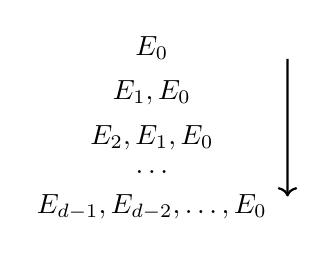
\begin{tikzpicture}[auto,node distance = 0cm and 0cm, thick]
    % Nodes
    \node(E0) {$E_0$};
    \node[below=of E0] (E1E0) {$E_1, E_0$};
    \node[right=of E0,xshift=1.25cm] (start){};
    \node[below=of E1E0] (E2E1E0) {$E_2, E_1, E_0$};
    \node[below=of E2E1E0] (E3E2E1E0) {$\ldots$};
    \node[below=of E3E2E1E0] (Ed1Ed2E0) {$E_{d-1}, E_{d-2}, \ldots, E_0$};
    \node[right=of Ed1Ed2E0,xshift=0cm] (end){};

    \draw[->] (start) -- (end);
\end{tikzpicture}
\caption{Bitonic Sorting Paradigm execution schema}
\end{figure}

\subsubsection{Bitonic Sorting Paradigm Implementation}
Based on the Bitonic Sorting Paradigm, the implementation can be summarized as follows:
\begin{enumerate}
    \item Divide the dataset into $P$ equal parts, assigning one part to each processor.
    \item Use the Merge Sort routine to sort each subset locally on its respective processor.
    \item Employ the Bitonic Sorting Paradigm on a virtual hypercube with  $\log_2(P)$ dimensions.
    During each stage:
    \begin{itemize}
        \item Merge sorted sequences from adjacent processors, where one processor merges sequences from the lower index and the other from the higher index.
        \item Continue merging until each processor's sequence reaches the middle point. 
    \end{itemize}
\end{enumerate}

\begin{figure}[thpb]
      \centering
      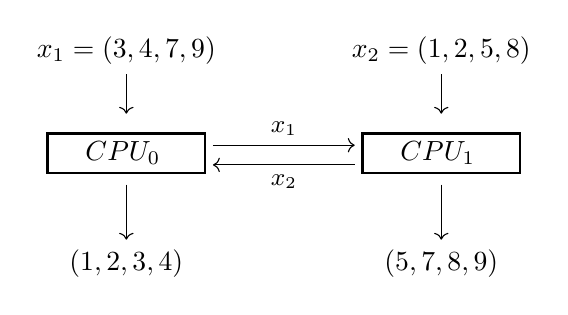
\begin{tikzpicture}
    
    % Draw the arrows
    \draw[->] (0,2) -- (0,1.5) node[at start,above]{$x_1=(3,4,7,9)$};
    \draw[thick] (-1,0.75) rectangle (1,1.25) node[at start, right, xshift=0.35cm,yshift=0.25cm]{$CPU_0$};
    \draw[->] (4,2) -- (4,1.5) node[at start,above]{$x_2=(1,2,5,8)$};
    \draw[thick] (3,0.75) rectangle (5,1.25) node[at start, right, xshift=0.35cm,yshift=0.25cm]{$CPU_1$};
    \draw[->] (1.1,1.1) -- (2.9,1.1) node[midway, above,font=\small]{$x_1$};
    \draw[->] (2.9,0.85) -- (1.1,0.85) node[midway, below,font=\small]{$x_2$};
    \draw[->] (4,0.6) -- (4,-0.1) node[at end,below]{$(5,7,8,9)$};
    \draw[->] (0,0.6) -- (0,-0.1) node[at end,below]{$(1,2,3,4)$};
\end{tikzpicture}
\caption{Bitonic Merging on 2 processors}
\end{figure}
This approach minimizes inter-processor communication while maximizing parallelism. It is worth noting that the sorting routine used in the initial phase can be tailored to the specific processor type, ensuring compatibility without disrupting the overall computational framework.
\begin{algorithm}[h]
\caption{Bitonic Sort}
\KwIn{Array $A$, Processor Set $P$}
\KwOut{Sorted array $A$}
\vspace{0.25em}
\SetAlgoLined
\SetKwFunction{FBitSort}{BitonicSort}
\SetKwFunction{FMergeL}{MergeLow}
\SetKwFunction{FMergeH}{MergeHigh}
\SetKwProg{Fn}{Function}{:}{}

\Fn{\FBitSort{$A$, $P$}}{
    \tcp{Scatter $A$ across $P$ processors}
    $A_0, A_1, \dots, A_{P-1}$\;
    
    \tcp{Execute in parallel on each processor $p \in \{0,\dots,P-1\}$}
    \FMain{$A_p$, $0$, $|A_p|- 1$}\;
    
    \For{$l \gets 0$ \KwTo $(\log_2{P})-1$}{
        \For{$i \gets l$ \KwTo $0$ \KwSty{step} $-1$}{
            $pal \gets \text{partner}(p, i, l)$\;
            $A_r \gets \text{data\_from}(pal)$\; \tcp{Exchange data between $p$ and $pal$}
            
            \If{$p$ merges from low index}{
                \FMergeL{$A_p$, $A_r$}\;
            }
            \Else{
                \FMergeH{$A_p$, $A_r$}\;
            }
        }
    }
    \tcp{Gather $A_p$ from each processor $p$}
    $A \gets A_0 \cup A_1 \cup \dots \cup A_{P-1}$\;
}
\end{algorithm}

%%%%%%%%%%%%%%%%%%%%%%%%%%%%%%%%%%%%%%%%%%%%%%%%%%%%%%%%%%%%%%%%%%%%%%%%%%%%%%%%

\section{Intended experiments}
The sequential MergeSort algorithm is implemented in C, while the BitonicSort algorithm is executed using MPI. The code and all implementation details are available on \textbf{\href{https://github.com/francesco-biscaccia-carrara/BitonicSort}{GitHub}}. \par
For simplicity, the algorithm is tested on datasets whose sizes are powers of two, with the number of processors also being a power of two. This simplification can be mitigated using padding strategies, which become less significant as the dataset size increases. Thus, this approach remains relevant and effective for larger datasets.
The tests include 10 measurements of both computation and communication time for each input size, with the datasets generated randomly for each measurement. Below are the input sizes used:
\begin{center}
\begin{tabular}{|c||c|}
 \hline
 \multicolumn{2}{|c|}{Instance Size} \\
 \hline
 Power of 2& Decimal\\
 \hline
 $2^{25}$ & $33554432$\\
 $2^{26}$ & $67108864$\\
 $2^{27}$ & $134217728$\\
 $2^{28}$ & $268435456$\\
 $2^{29}$ & $536870912$\\
 $2^{30}$ & $1073741824$\\
 \hline
\end{tabular}
\end{center}
All tests were performed on the \textbf{\href{https://capri.dei.unipd.it}{CAPRI}} High-Performance Computing (HPC) system, owned by the University of Padova. CAPRI is designed to provide computational power for testing innovative algorithms across various research fields. It is equipped with the following hardware:
\begin{itemize}
    \item 16 Intel(R) Xeon(R) Gold 6130 @ 2.10GHz CPUs
    \item 6 TB of RAM
    \item 2 NVIDIA Tesla P100 16GB GPUs
    \item 40 TB of disk space
\end{itemize}

The objective of these tests is to verify that the parallelization approach improves computing time while keeping communication time as a low percentage of the overall execution time. 
\par
To evaluate this, the sequential MergeSort was run for each input size 10 times, and the average computation time for each size is referred to as $T_{Seq}$.
Subsequently, the BitonicSort algorithm was executed on 2 to 32 processors, with the number of processors being powers of 2. For each configuration, the average computation time was measured similarly to the sequential tests, and the speedup$$S(P) = \frac{T_{Seq}}{T(P)}$$ was analyzed, where $T(P)$ is the execution time of the algorithm on $P$ processors.
Finally, the Computing-over-Communication Ratio (CCR) was evaluated, defined as $$CCR(P) = \frac{T_{Calc}(P)}{T_{Tot}(P)}$$ where $T_{Calc}(P)$ is the time devoted to computation, and $T_{Tot}(P)$ is the total execution time of the algorithm.

\addtolength{\textheight}{-12cm}   % This command serves to balance the column lengths
                                  % on the last page of the document manually. It shortens
                                  % the textheight of the last page by a suitable amount.
                                  % This command does not take effect until the next page
                                  % so it should come on the page before the last. Make
                                  % sure that you do not shorten the textheight too much.

%%%%%%%%%%%%%%%%%%%%%%%%%%%%%%%%%%%%%%%%%%%%%%%%%%%%%%%%%%%%%%%%%%%%%%%%%%%%%%%%
\vspace{\fill}
\printbibliography
%%%%%%%%%%%%%%%%%%%%%%%%%%%%%%%%%%%%%%%%%%%%%%%%%%%%%%%%%%%%%%%%%%%%%%%%%%%%%%%%
% WHAT MIGHT BE ADDED IN THE NEXT UPDATE PROPOSAL 
% --> list of analytical test to be conducted 
% --> in case the fact that the GAT cannot compute directed graphs
% --> more local graph features that came up to our mind
% --> everything that will be modified (DAHHH)
\end{document}